\documentclass[10pt, a4paper]{article}
\usepackage{amsmath}
\usepackage{amssymb}
\usepackage{mathtools}
\usepackage{mathtext}
\usepackage[T1, T2A]{fontenc}
\usepackage[utf8]{inputenc}
\usepackage[english, russian]{babel}
\usepackage{cmap}
\usepackage{fancyhdr}
\usepackage[pdftex]{graphicx}
\usepackage{gensymb}
\usepackage{floatrow}
\usepackage{titlesec}
\usepackage{lastpage}
\usepackage{float}
\usepackage{gensymb}
\usepackage{booktabs}
\usepackage{mathrsfs}
\usepackage{floatflt}
\usepackage{wrapfig}
\usepackage{caption}


\usepackage[figurename=Рис.]{caption}

\pagestyle{fancy}
	\fancyhf{}
	\lhead{\hspace{1bp} Работа \textnumero 4.7.1}
	\rhead{Терехов Максим 876\hspace{1bp}}
	\lfoot{Двойное лучепреломление}
	\cfoot{\textbf{}}
	\rfoot{\thepage\ \textnormal{из}\ \pageref{LastPage}}
	\renewcommand{\headrulewidth}{1pt}
	\renewcommand{\footrulewidth}{1pt}


%\addtolength{\hoffset}{-1.75cm}
%\addtolength{\textwidth}{3.5cm} 

%\addtolength{\voffset}{-1.5cm}
%\addtolength{\textheight}{3cm} 

\titleformat{\section}
    [block]{\normalfont\bfseries\Large}{\rlap{\thesection}}{0em}
    {\vspace{-0.02\textwidth}\begin{minipage}[t]{.95\textwidth}}
[\end{minipage}]


\thispagestyle{fancy}

\captionsetup{justification=centering}



\begin{document}
\selectlanguage{russian}
\huge
\begin{center}
\textbf{Двойное лучепреломление}
\end{center}
\parindent=1cm
\large
	\section*{Цель работы}
	
 Изучение зависимости показателя преломления необыкновенной волны от направления в двоякопреломляющем кристалле; определение главных показателей преломления $n_0$ --- обыкновенной и $n_e$ --- необыкновенной волны в кристалле наблюдение эффекта полного внутреннего отражения.
	\section*{Оборудование}

	Гелий-неоновый лазер, вращающийся столик с неподвижным лимбом, призма из исландского шпата, поляроид.
	\section*{Экспериментальная установка}
\begin{figure}[H]
	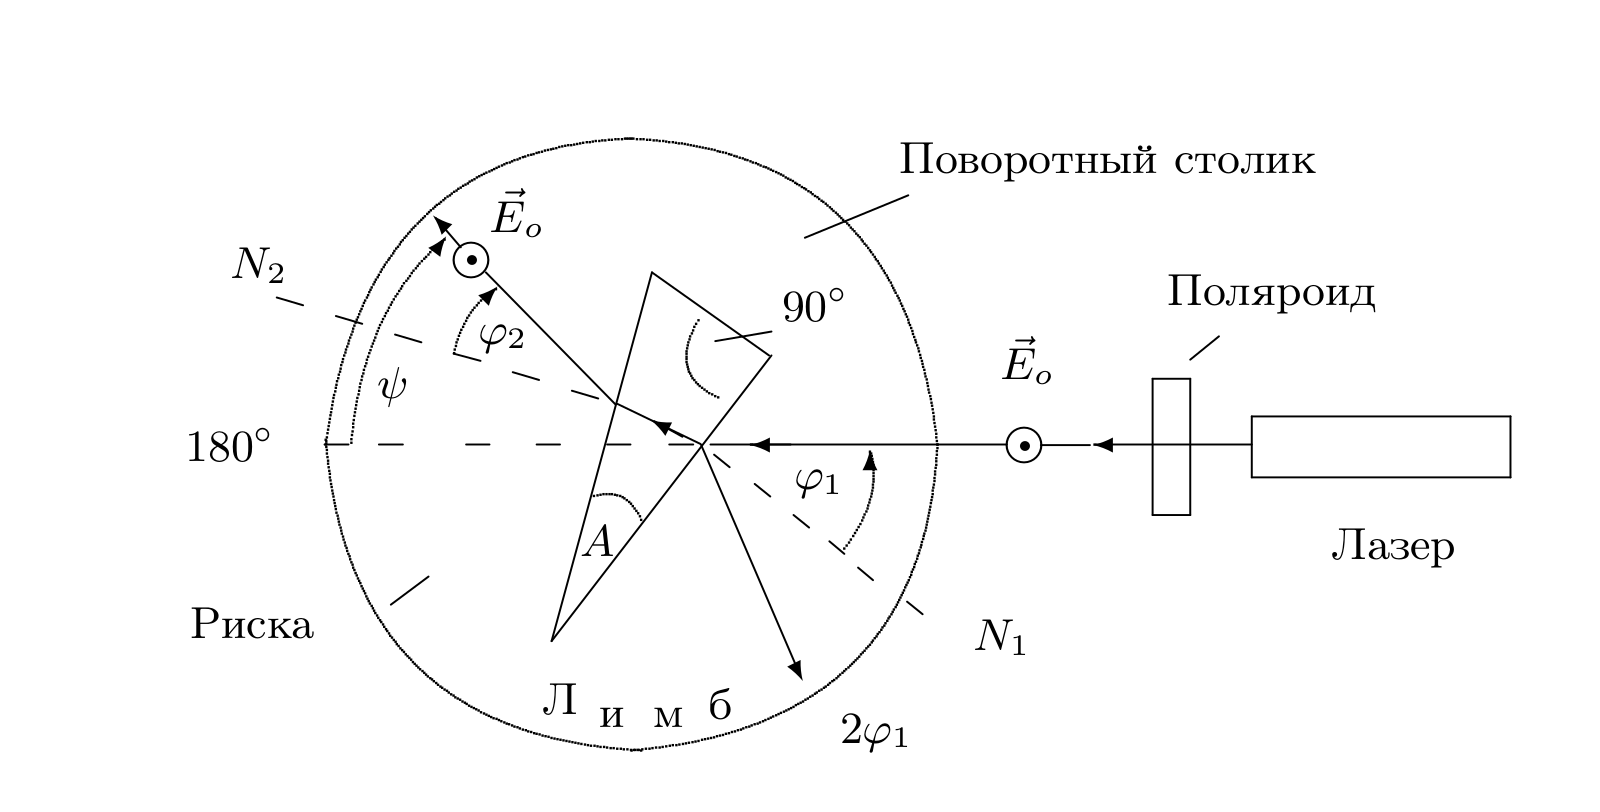
\includegraphics[width = 1.0\linewidth]{ust.png}
	\caption*{Схема экспериментальной установки}
\end{figure}	
\section*{Теоретическая часть}

При падении световой волны на границу изотропной среды в этой среде от границы распространяется одна волна. Если среда анизотропна, то в ней в общем случае возникают две волны, распространяющиеся от границы в разных направлениях и с разными скоростями. Это явление называется \textit{двойным лучепреломлением}.

\noindent \textbf{Плоские волны в кристаллах.} Фундаментальные уравнения Максвелла справедливы без всяких изменений и в кристаллических средах. В отсутствие электрических зарядов и токов они имеют вид
\begin{equation}
	\operatorname{rot} \vec{H}=\frac{1}{c} \frac{\partial \vec{D}}{\partial t}, \quad \operatorname{rot} \vec{E}=-\frac{1}{c} \frac{\partial \vec{B}}{\partial t}.
\end{equation}
Если среды прозрачны и однородны, то в них могут распространяться
плоские монохроматические волны. Запишем такую волну в комплексном виде:
\[
\vec{E}=\vec{E}_{0} e^{i(\omega t-\vec{k} \vec{r})} ; \quad \vec{B}=\vec{H}=\vec{H}_{0} e^{i(\omega t-\vec{k} \vec{r})} ; \quad \vec{D}=\vec{D}_{0} e^{i(\omega t-\vec{k} \vec{r})}.
\]
Здесь $\omega$ --- круговая частота, $\vec k$ --- волновой вектор, а амплитуды $\vec E_0$, $\vec H_0$, $\vec D_0$ постоянны. Вектор $\vec B$ совпадает с $\vec H$, так как $\mu = 1$. Дифференцируя по времени, получаем $\partial \vec D / \partial t = i \omega \vec D$, то есть операци дифференцирования сводится в этом случае к умножению на $i \omega$. Аналогично дифференцирование по координатам $x, y, z$ сводится к умножению на $- i k_x, -i k_y, -i k_z$. Заметив это и обозначив координатные орты через $\vec e_x, \vec e_y, \vec e_z$, получаем

\begin{equation*}
\operatorname{rot} \vec{H}=\left|\begin{array}{ccc}
\vec{e}_{x} & \vec{e}_{y} & \vec{e}_{z} \\
\frac{\partial}{\partial x} & \frac{\partial}{\partial y} & \frac{\partial}{\partial z} \\
H_{x} & H_{y} & H_{z}
\end{array}\right|=-i\left|\begin{array}{ccc}
\vec{e}_{x} & \vec{e}_{y} & \vec{e}_{z} \\
k_{x} & k_{y} & k_{z} \\
H_{x} & H_{y} & H_{z}
\end{array}\right|=-i[\vec{k} \vec{H}]
\end{equation*}
 и аналогично для $\operatorname{rot} \vec E $. В результате (1) перейдут в
 \[
 	\left[ \vec k \vec H \right] = - \frac{\omega}{c} \vec D; \quad \left[ \vec k \vec E \right] = \frac{\omega}{c} \vec B.
 \]
 Введем единичный вектор нормали $\vec N$ к фронту волны и скорость распространения фронта в направлении этой нормали $v$. Тогда $\vec k = \frac{\omega}{c} \vec N$ и предыдущие соотношения перейдут в
 \begin{equation}
 	\vec D = \frac{c}{v} \left[ \vec N \vec H \right]; \quad \vec B = \frac{c}{v} \left[ \vec N \vec E \right].
 \end{equation}
 Отсюда видно, что векторы $\vec D, \vec H, \vec N$ взаимно перпендикулярны. Значит, плоские волны в кристалле поперечны в отношении векторов $\vec D$ и $\vec H$. Однако в общем случае они не поперечны в отношении вектора $\vec E$.
 \newpage 
 

\begin{wrapfigure}{r}{0.45\textwidth}
    \centering
    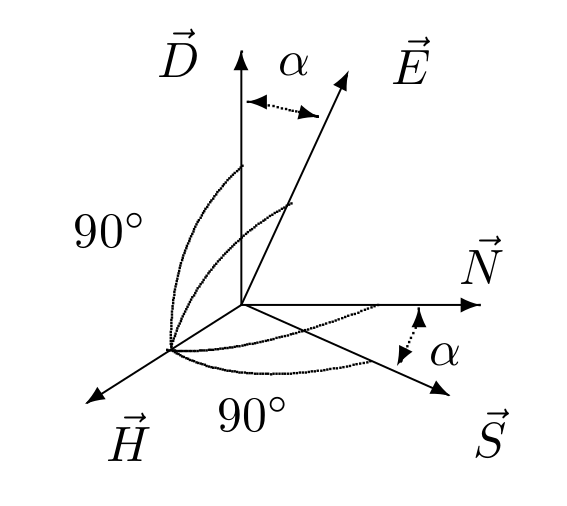
\includegraphics[width=1\textwidth]{DENS.png}
    \caption{Расположение векторов $\vec D, \vec E, \vec N, \vec S$ в анизотропной среде}
\end{wrapfigure} 
 
 
 В изотропной среде связь между вектором напряженности электрического поля $\vec E$ и вектором индукции $\vec D$ дается материальным уравнением $\vec D = \varepsilon \vec E$, где $\varepsilon$ --- постоянная, не зависящая от направления величина, называемая диэлектрической проницаемостью. Для характеристики оптических свойств анизотропной среды требуется девять величин $\varepsilon_{i j}$, образующих тензор диэлектрической проницаемости. Он вводится посредством отношений
 \begin{equation}
 	D_i = \sum_j \varepsilon_{i j} E_j \quad (i, j = x, y, z).
 \end{equation}
 Блягодаря тензорной связи между $\vec D$ и $\vec E$ направления этих векторов в кристаллах, вообще говоря, не совпадают. Плоскость $\left( \vec E, \vec H \right)$ обладает тем свойством, что перпендикуляр к ней определяет направление вектора Пойнтинга $\vec S = \frac{c}{4 \pi} \left[\vec E \vec H \right]$, то есть направление распространения световых лучей. Четыре вектора $\vec D, \vec E, \vec N, \vec S$ лежат в одной плоскости, перпендикулярной вектору $\vec H$. Взаимное расположение этих векторов показано на рис. 1.

\noindent \textbf{Оптически одноосные кристаллы.} Всю совокупность возможных значений тензора диэлектрической проницаемости можно представить при помощи трехосного эллипсоида. Значение диэлектрической проницаемости для любого направления выражается длиной радиуса-вектора эллипсоида, проведенного по этому направлению. Три значения диэлектричеcкой проницаемости $\varepsilon_x, \varepsilon_y, \varepsilon_z$, соответствующие осям эллипсоидв, называются \textit{главными значениями диэлектрической проницаемости} и соответственно $\sqrt{\varepsilon_x}, \sqrt{\varepsilon_y}, \sqrt{\varepsilon_z}$ --- \textit{главными показателями преломления}.

В системе координат, оси которой совпадают с главными осями эллипсоида, тензор диэлектрической проницаемости приводится к диагональному виду, и проекции векторов $D$ и $E$ на оси координат связаны простыми соотношениями:
\begin{equation*}
	D_x = \varepsilon_x E_x, \quad D_y = \varepsilon_y E_y, \quad D_z = \varepsilon_z E_z.
\end{equation*}

В оптически одноосном кристалле, каковым является исландский шпат, эллипсоид диэлектрической проницаемости представляет собой эллипсоид вращения.
В нём оптическая ось совпадает с осью вращения эллипсоида диэлектрических проницаемостей. Для главных значений диэлектрических проницаемостей приняты обозначения $\varepsilon_z = \varepsilon_\parallel$ и $\varepsilon_x = \varepsilon_y = \varepsilon_\perp$. В дальнейшем нам потребуется связь между проекциями векторов $\vec D$ и $\vec E$ на оптическую ось кристалла $(\vec D_\parallel $ и $\vec E_\parallel )$ и на плоскость, перпендикулярную оси $(\vec D_\perp $ и $\vec E_\perp )$:
\begin{equation}
	\vec D_\parallel  = \varepsilon_\parallel \vec E_\parallel , \quad \vec D_\perp  = \varepsilon_\perp \vec E_\perp. 
\end{equation}

\begin{wrapfigure}{r}{0.45\textwidth}
    \centering
    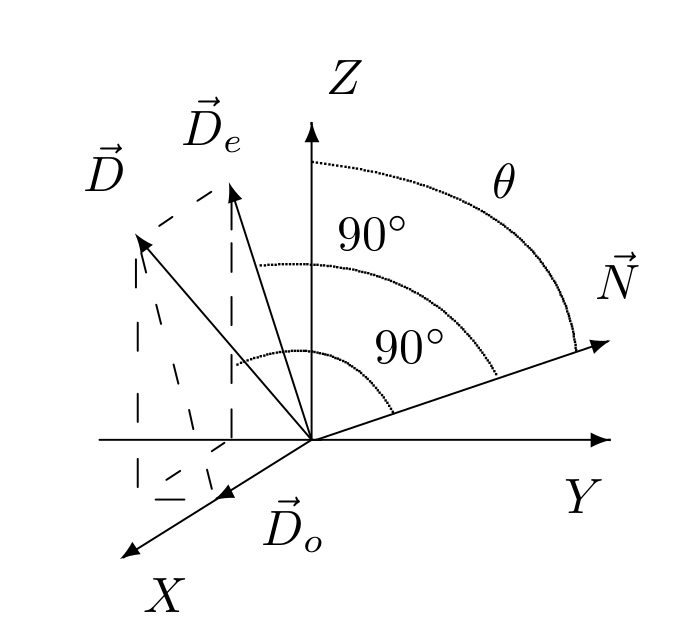
\includegraphics[width=1\textwidth]{DN.png}
    \caption{Расположение векторов $\vec N$ и $\vec D$ в анизотропной среде: $(\vec D = \vec D_o + \vec D_e; \vec D_o \perp \vec D_e; \vec D \perp \vec N);$ $\vec N$ и $\vec D_e$ лежат в плоскости $(Z, Y)$; $\vec D_o$ перпендикулярен плоскости $(Z, Y)$}
\end{wrapfigure} 
Волну, распространяющуюся в одноосном кристалле, можно разделить на две линейно поляризованные волны: обыкновенную, вектор электрической индукции $\vec D_o$ которой перпендикулярен главному сеению, и необыкновенную, с вектором электрической индукции $\vec D_e$, лежащим в главном сечении (рис. 2) \textit{Главным сечением кристалла} называется плоскость, в которой лежит оптическая ось кристалла и нормаль к фронту волны.

Рассмотрим вначале обыкновенную волну, которой вектор $\vec D_o$ перпендикулярен главному сечению. Тогда $D_{oz} = 0$, и из условия $D_z = \varepsilon_z E_z$ следует, что $E_{oz} = 0.$ Кроме того, так как $D_{oy} = \varepsilon_\perp E_{oy}$ и $D_{ox} = \varepsilon_\perp E_{ox}$, то можно записать 
\begin{equation}
	\vec D_o = \varepsilon_\perp \vec E_o.
\end{equation}

Таким образом, для обыкновенной волны материальное уравнение
имеет такой же вид, как и в изотропной среде. Найдем с помощью этого
уравнения скорость распространения обыкновенной волны и соответ-
ствующий показатель преломления. Из (2) имеем
\[
	D_o = \frac{c}{v_o} H_o, \quad H_o = \frac{c}{v_o} E_o
\]
или, учитывая (5),
\[
	\varepsilon_{\perp} E_o = \frac{c}{v_o} H_o, \quad H_o = \frac{c}{v_o} E_o,
\]
откуда
\[
	v_o = \frac{c}{ \sqrt{\varepsilon_{\perp}}} \quad \text{и} \quad n_o = \frac{c}{v_o} = \sqrt{\varepsilon_\perp}.
\]
Таким образом, скорость распространения обыкновенной волны и ее показатель преломления не зависят от направления распространения.

У необыкновенной волны вектор $\vec D_e$ не параллелен $\vec E_e$, и связь между ними сложнее, чем в (5).

Для того чтобы найти скорость распространения $v$ и показатель преломления нобыкновенной волны $n = c / v$, достаточно найти связь между вектором электрической индукции этой волны $\vec D_e$ и проекцией на него вектора электрического поля волны $E_{eD}$. Тогда, подставляя $D_e = \varepsilon E_{eD}$ в (2), приходим к соотношения
\[
	\varepsilon E_{eD} = \frac{c}{v} H_e; \quad H_e = \frac{c}{v} E_{eD},
\]
формально тождественным с соотношениями для обыкновенной волны. Роль величины $\varepsilon_\perp$ тперь играет величина $\varepsilon$, а показатель преломления необыкновеной волны равен $\sqrt{\varepsilon}$.

Найдём связь между $D_e$ и $E_{eD}$. Для этого разложим векторы $\vec D_e$ и $\vec E_e$ на составляющие, параллельные и перпендикулярные оси кристалла:
\[
	\vec D_e = \vec D_{e \parallel} + \vec D_{e \perp}.
\]
\[
	\vec E_e = \vec E_{e \parallel} + \vec E_{e \perp}.
\]
Учитывая (4), находим
\[
	E_{eD} = \frac{\vec E_e \vec D_e}{D_e} = \frac{E_{e \parallel} D_{e \parallel} + E_{e \perp} D_{e \perp}}{D_e} = \frac{D^2_{e \parallel} / \varepsilon_\parallel + D^2_{e \perp} / \varepsilon_\perp}{D_e}
\]
или 
\[
E_{eD} = D_e \left( \frac{\sin^2{\theta}}{\varepsilon_\parallel} + \frac{\cos^2{\theta}}{\varepsilon_\perp} \right) = \frac{D_e}{\varepsilon},
\]
где $\theta$ "--- угол между оптической осью $Z$ и волновой нормалью $N$:
\begin{equation}
	\sin \theta = \frac{D_{e \parallel}}{D_e}, \quad \cos \theta = \frac{D_{e \perp}}{D_e}.
\end{equation}
Таким образом, $\varepsilon$ и соответственно скорость распространения и показатель преломления необыкновенной волны зависят от угла между оптической осью кристалла и   направлением распространения волны.

Выпишем выражение для показателя преломления необыкновенной волны $n = \sqrt \varepsilon$ через главные показатели преломления $n_o, n_e$ и угол $\theta$:
\begin{equation}
	\frac{1}{\left[ n(\theta) \right] ^ 2} = \frac{\sin^2 \theta}{n^2_e} + \frac{\cos^2 \theta}{n^2_o}.
\end{equation}
При $n_o - n_e \ll n_o$ и $n_e$ (для исландского шпата $n_o = 1,655, n_e = 1,485$ для $\lambda = 0,63$ мкм) (7) можно упростить:
\begin{equation}
	n(\theta) \approx n_e + (n_o - n_e) \cos^2 \theta.
\end{equation}

\noindent \textbf{Двойное лучепреломление в призме из исландского шпата.} Рассмотрим, как по преломлению лучей в кристаллической призме можно определить показатели преломления для обыкновенной и необыкновенной волны. В работе исследуется одна из двух призм, составляющих поляризатор (рис. 3).
\begin{figure}[H]
	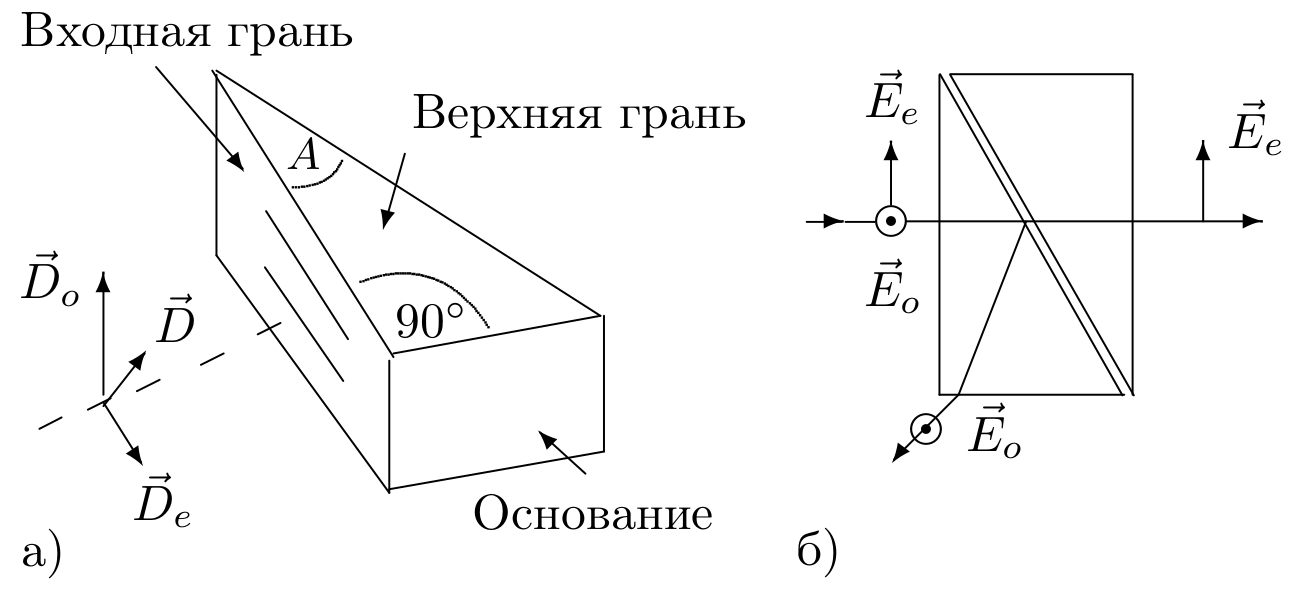
\includegraphics[width = 1.0\linewidth]{shpat.png}
	\caption{ а) Исследуемая призма из исландского шпата. Штриховкой указано направление оптической оси кристалла. б) Ход лучей в поляризационной призме}
\end{figure}	
В исследуемой призме ось кристалла лежит в плоскости, параллельной верхней грани призмы, причем она параллельна входной грани призмы (длинному катету). При этом в обыкновенной волне вектор $\vec D_o$ пендикулярен верхней грани призмы, а в необыкновенной волне вектор $\vec D_e$  параллелен верхней грани.
\begin{wrapfigure}{r}{0.45\textwidth}
    \centering
    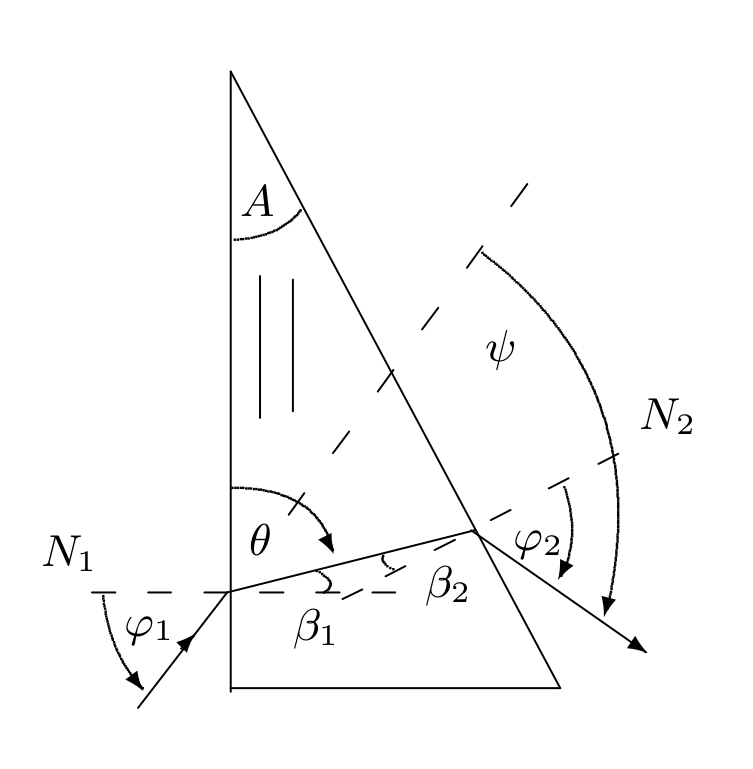
\includegraphics[width=1\textwidth]{prism.png}
    \caption{Ход лучей в призме}
\end{wrapfigure} 
Волну, падающую на входную грань призмы, можно представить в виде суммы двух ортогональных линейно поляризованных волн. Преломление этих двух волн на грани призмы можно рассматривать независимо. Волна, в которой вектор $\vec D$ направлен вертикально (перпендикулярно верхней грани и оси кристалла), внутри кристалла будет распространяться как обыкновенная. Для этой волны выполняется закон Снеллиуса, а показатель преломления призмы для нее равен $n_o$. Волна, в которой вектор $\vec D$ направлен горизонтально, в кристалле будет распространяться как необыкновенная. Для этой волны также будет выполняться закон Снеллиуса, но с тем отличием, что показатель преломления призмы для нее будет зависеть от угла между осью кристалла и волновой нормалью. 

Значение показателя преломления и угол, под которым преломилась волна в призме, можно найти, измерив угол падения на входную грань призмы $\phi_1$ и угол $\phi_2$ на выходе призмы (рис. 4). Запишем закон Снеллиуса для одной из волн применительно к первой и второй граням призмы:
\[
	\sin \phi = n \sin \beta_1;
\]
\[
	\sin \phi_2 = n \sin \beta_2 = n \sin (A - \beta_1).
\]
При этом мы выразили угол падения на вторую грань призмы $\beta_2$ через угол преломления на первой грани призмы $\beta_1$ и угол при вершине призмы $A$. Как видно из рис. 4, эти углы связаны простым соотношением $A = \beta_1 + \beta_2$. Учитывая, что угол преломления $\beta_1$ связан с углом $\theta$ между осью кристалла и волновой нормалью $\vec N$ соотношением $\theta + \beta_1 = \pi / 2$, находим $n$ и $\theta$:
\begin{equation}
n = \frac{1}{\sin A} \sqrt{\sin^2 \varphi_1 + \sin^2 \varphi_2 + 2 \sin \varphi_1 \sin \varphi_2 \cos A};
\end{equation}
\[
	\cos \theta = \frac{\sin \varphi_1}{n}.
\]
Для обыкновенной волны $n$ не будет зависеть от угла $\theta$, а для необыкновенной волны зависимость $n$ от $\theta$ должна описываться выражением (7).

Показатель преломления призмы из изотропного материала удобно находить по углу нименьшего отклонения луча от первоначального направления. Угол отклонения луча призмой ($\psi$ на рис. 4) минимален для симметричного хода лучей, то есть когда $\varphi_1 = \varphi_2$. Тогда показатель преломления можно рассчитать по формуле
\begin{equation}
n=\frac{\sin \left(\frac{\psi_{m}+A}{2}\right)}{\sin \left(\frac{A}{2}\right)},
\end{equation}
где $\psi_m$ --- угол наименьшего отклонения.

Если призма неизотропна, то этой формулой, строго говоря, можно воспользоваться только для обыкновенной волны, которая, как это было показано ранее, распространяется так же, как и в изотропной среде. Но если учесть, что угол при вершине призмы мал, и при угле наименьшего отклонения преломлённый луч в призме распространяется под углом к оси кристалла близким к $\pi / 2$, то в качестве оценки формулу (10) можно использовать для определения $n_e$.
	\section*{Обработка результатов экспериментов}
	Проведём основную серию измерений с шагом $2.5^o \text{--} 5^o$:
	\begin{table}[H]
	\centering
	\begin{tabular}{|c|c|c|c|c|c|c|c|c|c|c|c|}  \hline
	$2 \varphi_1$ & 9 & 13 & 18 & 20 & 24 & 28 & 32 & 35 & 40 & 46 & 49 \\\hline
	$2 \pi + \psi_e$ & 204.5 & 202.5 & 202 & 201.5 & 201 & 200.7 & 200.3 & 200 & 200 & 200 & 200 \\\hline
	$\sigma$ & 1.9 & 1.8 & 1.8 & 1.8 & 1.8 & 1.8 & 1.8 & 1.8 & 1.8 & 1.8 & 1.8 \\\hline
	$2\pi+ \psi_o$ & 216.5 & 214 & 212 & 211 & 210 & 209 & 208.5 & 208 & 207.3 & 206.9 & 206.6 \\\hline
	$\sigma$ & 2.2 & 2.1 & 2.1 & 2.1 & 2.1 & 2.1 & 2.1 & 2.1 & 2.1 & 2.1 & 2.1 \\\hline
	$\varphi_1$ & 4.5 & 6.5 & 9 & 10 & 12 & 14 & 16 & 17.5 & 20 & 23 & 24.5 \\\hline
	$\varphi_e$ & 24.5 & 22.5 & 22 & 21.5 & 21 & 20.7 & 20.3 & 20 & 20 & 20 & 20 \\\hline
	$\psi_o$ & 36.5 & 34 & 32 & 31 & 30 & 29 & 28.5 & 28 & 27.3 & 26.9 & 26.6 \\\hline
	$\phi_e$ & 57 & 53 & 50 & 48.5 & 46 & 43.7 & 41.3 & 39.5 & 37 & 34 & 32.5 \\\hline
	$\phi_o$ & 69 & 64.5 & 60 & 58 & 55 & 52 & 49.5 & 47.5 & 44.3 & 40.9 & 39.1 \\\hline
	$\cos^2 \theta \cdot 10^3$ & 3 & 6 & 11 & 14 & 20 & 26 & 34 & 41 & 52 & 68 & 76 \\\hline
	$n_e(\theta)$ & 1.50 & 1.48 & 1.49 & 1.49 & 1.49 & 1.49 & 1.50 & 1.49 & 1.49 & 1.50 & 1.50 \\\hline
	$cos^2(\theta) \cdot 10^3$ & 2 & 5 & 9 & 11 & 16 & 22 & 28 & 33 & 43 & 56 & 63 \\\hline
	$n_o (\theta)$ & 1.66 & 1.65 & 1.65 & 1.65 & 1.65 & 1.65 & 1.65 & 1.65 & 1.65 & 1.65 & 1.65 \\\hline
	\end{tabular}
	\end{table}
	\begin{figure}[H]
	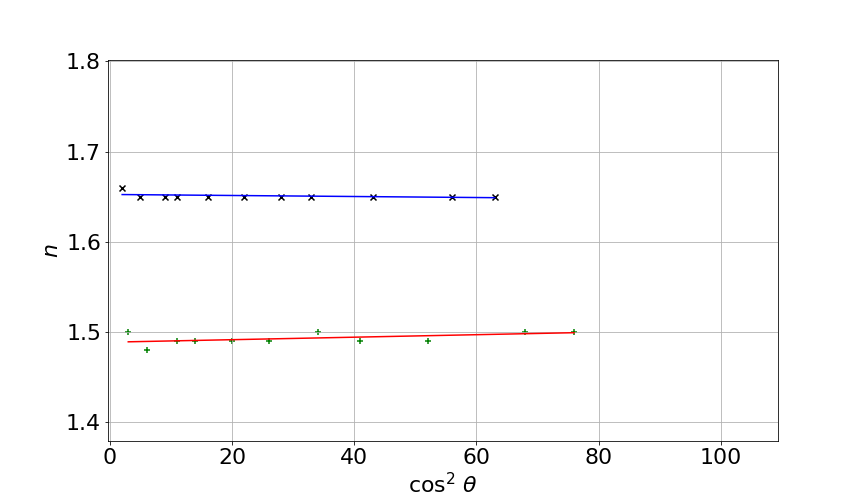
\includegraphics[width = 1.0\linewidth]{g1.png}
	\caption{Синяя "--- обыкновенная, красная "--- необыкновенная}
\end{figure}
\textbf{Расчёт показателей преломления на основании трёх экспериментов:}

Расчёт по обыкновенной и необыкновенной волне:
\[
	\text{При} \ A = 37^o \quad n_o = 1.65 \pm 0.01; \quad n_e = 1.49 \pm 0.03;
\] 
Расчёт по углу наименьшего отклонения:
\[
\varphi_o^m = 26.1 \pm 1; \quad \psi_e^m = 20 \pm 1.
\]
\[
	\text{При}\ A = 37^o \quad n_o = 1.64 \pm 0.003; \quad n_e = 1.50 \pm 0.04;
\]
Расчёт по углу поного внутреннего отражения:
\[
	\phi_o = (1 \pm 3)^o; \quad \phi_e = (-6.5 \pm 3)^o;
\]
\[
	n_o = 1.69 \pm 0.03; \quad n_e = 1.52 \pm 0.03.
\]
\section*{Вывод}
В работе были получены значения показателей преломления для обыкновенной и необыкновенной волн в исландсокм шпате тремя методами. Легко убедиться, что значения совпадают с теоретическими с учётом погрешностей. Теория подтверждена экспериментально.
\end{document}
